% Options for packages loaded elsewhere
\PassOptionsToPackage{unicode}{hyperref}
\PassOptionsToPackage{hyphens}{url}
\documentclass[
  11pt]{article}
\usepackage{xcolor}
\usepackage[margin=0.7in]{geometry}
\usepackage{amsmath,amssymb}
\usepackage{enumitem}
\setcounter{secnumdepth}{-\maxdimen} % remove section numbering
\usepackage{iftex}
\ifPDFTeX
  \usepackage[T1]{fontenc}
  \usepackage[utf8]{inputenc}
  \usepackage{textcomp} % provide euro and other symbols
\else % if luatex or xetex
  \usepackage{unicode-math} % this also loads fontspec
  \defaultfontfeatures{Scale=MatchLowercase}
  \defaultfontfeatures[\rmfamily]{Ligatures=TeX,Scale=1}
\fi
\usepackage{lmodern}
\ifPDFTeX\else
  % xetex/luatex font selection
\fi
% Use upquote if available, for straight quotes in verbatim environments
\IfFileExists{upquote.sty}{\usepackage{upquote}}{}
\IfFileExists{microtype.sty}{% use microtype if available
  \usepackage[]{microtype}
  \UseMicrotypeSet[protrusion]{basicmath} % disable protrusion for tt fonts
}{}
\makeatletter
\@ifundefined{KOMAClassName}{% if non-KOMA class
  \IfFileExists{parskip.sty}{%
    \usepackage{parskip}
  }{% else
    \setlength{\parindent}{0pt}
    \setlength{\parskip}{6pt plus 2pt minus 1pt}}
}{% if KOMA class
  \KOMAoptions{parskip=half}}
\makeatother
\usepackage{longtable,booktabs,array}
\usepackage{calc} % for calculating minipage widths
% Correct order of tables after \paragraph or \subparagraph
\usepackage{etoolbox}
\makeatletter
\patchcmd\longtable{\par}{\if@noskipsec\mbox{}\fi\par}{}{}
\makeatother
% Allow footnotes in longtable head/foot
\IfFileExists{footnotehyper.sty}{\usepackage{footnotehyper}}{\usepackage{footnote}}
\makesavenoteenv{longtable}
\usepackage{graphicx}
\usepackage{float}
\makeatletter
\newsavebox\pandoc@box
\newcommand*\pandocbounded[1]{% scales image to fit in text height/width
  \sbox\pandoc@box{#1}%
  \Gscale@div\@tempa{\textheight}{\dimexpr\ht\pandoc@box+\dp\pandoc@box\relax}%
  \Gscale@div\@tempb{\linewidth}{\wd\pandoc@box}%
  \ifdim\@tempb\p@<\@tempa\p@\let\@tempa\@tempb\fi% select the smaller of both
  \ifdim\@tempa\p@<\p@\scalebox{\@tempa}{\usebox\pandoc@box}%
  \else\usebox{\pandoc@box}%
  \fi%
}
% Set default figure placement to htbp
\def\fps@figure{htbp}
\makeatother
\setlength{\emergencystretch}{3em} % prevent overfull lines
\providecommand{\tightlist}{%
  \setlength{\itemsep}{0pt}\setlength{\parskip}{0pt}}
\usepackage{bookmark}
\IfFileExists{xurl.sty}{\usepackage{xurl}}{} % add URL line breaks if available
\urlstyle{same}
\hypersetup{
  hidelinks,
  pdfcreator={LaTeX via pandoc}}

\usepackage{braket}
\usepackage{wasysym}
\newcommand{\pts}[1]{\hfill{\small\bfseries(#1 pts)}}
\newcounter{problem}
\newcommand{\problem}[2]{%
  \refstepcounter{problem}%
  \vspace{10pt}\noindent\textbf{Problem \theproblem.~#1}\pts{#2}\par
}

\newcounter{bonus}
\newcommand{\bonus}[2]{%
  \refstepcounter{bonus}%
  \vspace{10pt}\noindent\textbf{Bonus \Alph{bonus}.~#1}\pts{#2}\par
}
\newcommand{\pagereferences}[1]{%
  \vfill
  \noindent\rule{\textwidth}{0.3pt}\par
  {\scriptsize\textbf{References by part:} #1\par}
}

\author{Piter Garcia}
\date{October 6, 2026}

\begin{document}

\title{CSCI-739 Quantum Machine Learning\\[2pt]
\large Homework 1 --- Expert-Assessment Version}
\maketitle

\textbf{Basis convention:} written kets use \(\lvert q_0q_1\cdots\rangle\); Qiskit count strings are mapped explicitly below. The \href{./Homework_1-Comprehensive-Learning-Reference.md}{comprehensive reference} gives the extended derivations and \href{./Homework_1-Qiskit-Verification.ipynb}{verification notebook} contains runnable circuits.

\problem{Qubit Basics}{10}\label{problem-1-qubit-basics}

\textbf{Given:} a general single-qubit state \(\ket{\psi}=\alpha\ket{0}+\beta\ket{1}\), with \(\alpha,\beta\in\mathbb C\) and \(|\alpha|^2+|\beta|^2=1\).

\begin{figure}
\centering
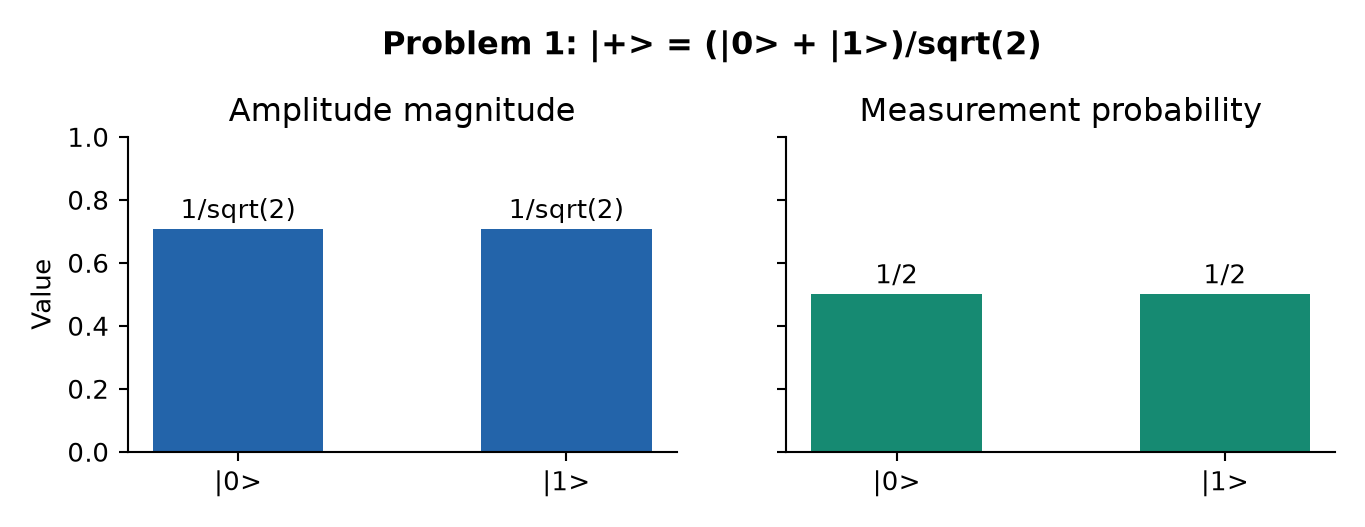
\includegraphics[width=0.84\textwidth]{./figures/problem1_amplitude_probability.png}
\caption{Equal-superposition amplitude magnitudes and measurement probabilities; the magnitude is squared to obtain probability.}
\end{figure}

\small
\begin{enumerate}[label=\textbf{(\alph*)},leftmargin=*,itemsep=2pt,topsep=2pt,parsep=0pt]
\item \textbf{Question.} Write the expression for the probability of measuring the qubit in the state \(\ket{0}\) and in the state \(\ket{1}\), using inner products (bra-ket notation).\\
\textbf{Answer.} For \(\lvert\psi\rangle=\alpha\lvert0\rangle+\beta\lvert1\rangle\), \(\langle0|\psi\rangle=\alpha\) and \(\langle1|\psi\rangle=\beta\); hence \(P(0)=|\alpha|^2\) and \(P(1)=|\beta|^2\).
\item \textbf{Question.} Verify that the sum of the two probabilities is always equal to \(1\).\\
\textbf{Answer.} The normalization condition gives \(P(0)+P(1)=|\alpha|^2+|\beta|^2=1\), equivalently \(\langle\psi|\psi\rangle=1\).
\item \textbf{Question.} For the specific state \(\ket{\psi}=\tfrac{1}{\sqrt{2}}\ket{0}+\tfrac{1}{\sqrt{2}}\ket{1}\), calculate explicitly the probability of obtaining \(\ket{0}\) and of obtaining \(\ket{1}\).\\
\textbf{Answer.} Each amplitude has magnitude \(1/\sqrt2\), so \(P(0)=P(1)=1/2\). One measurement returns one outcome; these probabilities describe repeated measurements.
\end{enumerate}
\normalsize
\pagereferences{(a)--(c): QML0 / Lecture 1, slides 33--39 (complex amplitudes, Dirac notation, Born rule, normalization).}

\newpage
\problem{Two-Qubit Systems and CNOT}{15}\label{problem-2-two-qubit-systems-and-cnot}

\begin{figure}[H]
\centering
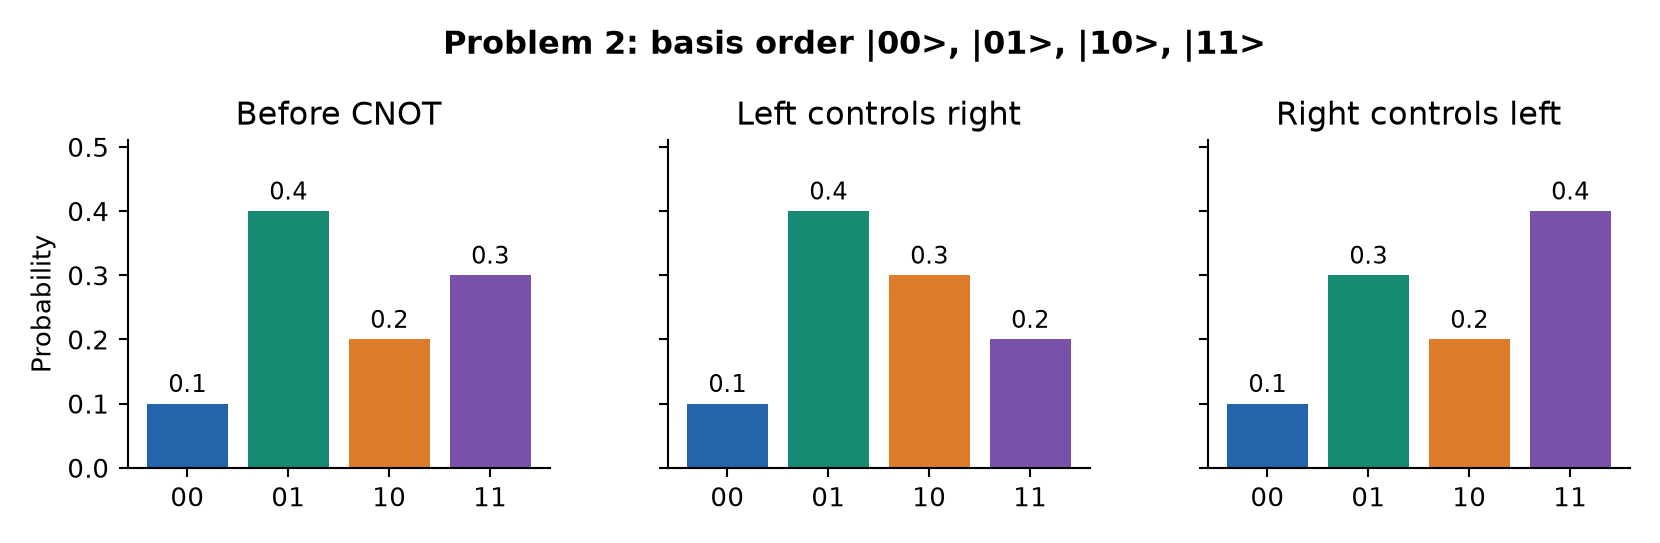
\includegraphics[width=0.84\textwidth]{./figures/problem2_cnot_probabilities.png}
\caption{Exact computational-basis probabilities before CNOT and after each control direction.}
\end{figure}

\small
\begin{enumerate}[label=\textbf{(\alph*)},leftmargin=*,itemsep=2pt,topsep=2pt,parsep=0pt]
\item \textbf{Question.} Define each of the four basis states \(\ket{00}, \ket{01}, \ket{10}, \ket{11}\) explicitly using tensor product notation between single-qubit states, and then write the vector representation of each of the four basis states.\\
\textbf{Answer.} In order \((00,01,10,11)\), the states are \(\ket{0}\otimes\ket{0},\ket{0}\otimes\ket{1},\ket{1}\otimes\ket{0},\ket{1}\otimes\ket{1}\); their vectors are \((1,0,0,0)^T,(0,1,0,0)^T,(0,0,1,0)^T,(0,0,0,1)^T\).
\item \textbf{Question.} Consider the two-qubit state \(\ket{\psi}=\sqrt{\tfrac{1}{10}}\ket{00}+\sqrt{\tfrac{4}{10}}\ket{01}+\sqrt{\tfrac{2}{10}}\ket{10}+\sqrt{\tfrac{3}{10}}\ket{11}\). Verify normalization and state the probability of each basis outcome. \textit{Note: In this example the amplitudes are real, but in general they are complex, and the probability is the modulus squared of the amplitude.}\\
\textbf{Answer.} The squared norm is \((1+4+2+3)/10=1\); probabilities in the stated order are \((1,4,2,3)/10\).
\item \textbf{Question.} Compute the probability of measuring each basis state after applying a CNOT gate with the left qubit as control and the right as target.\\
\textbf{Answer.} The map is \(00\to00,\ 01\to01,\ 10\to11,\ 11\to10\). It exchanges the last two amplitudes, so the probabilities become \((1,4,3,2)/10\).
\item \textbf{Question.} Derive the \(4\times4\) unitary matrix of the flipped-control CNOT (right controls, left is target). \textit{Hint:} track where each basis state maps under this assumption, and create a unitary matrix that would map each basis state to the expected operation.\\
\textbf{Answer.} Since \(\ket{ab}\mapsto\ket{a\oplus b,b}\), the map is \(00\to00,\ 01\to11,\ 10\to10,\ 11\to01\), giving
\[
U_{R\to L}=\begin{pmatrix}1&0&0&0\\0&0&0&1\\0&0&1&0\\0&1&0&0\end{pmatrix}.
\]
\item \textbf{Question.} Prove that the matrix in (d) is unitary.\\
\textbf{Answer.} This real symmetric matrix swaps \(01\leftrightarrow11\) and fixes the other basis states. Thus \(U^\dagger=U\), \(U^2=I_4\), and \(U^\dagger U=I_4\).
\end{enumerate}
\normalsize
\pagereferences{(a)--(e): QML0 / Lecture 1, slides 40--45 and 54 (tensor bases, CNOT action, unitarity).}

\newpage
\problem{Bloch Sphere and Single-Qubit Gates}{20}\label{problem-3-bloch-sphere-and-single-qubit-gates}

\begin{figure}[H]
\centering
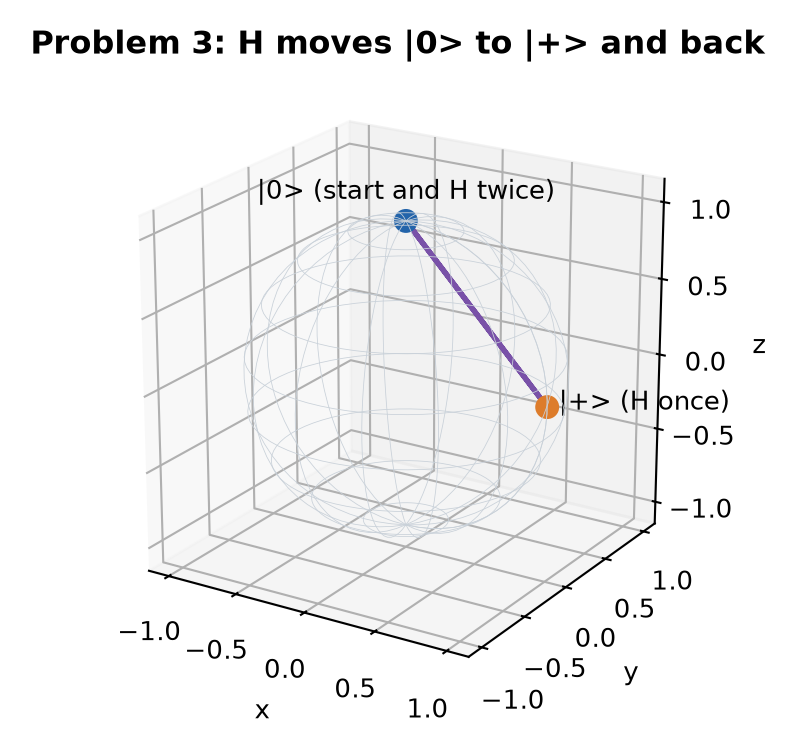
\includegraphics[width=0.58\textwidth]{./figures/problem3_hadamard_bloch.png}
\caption{Bloch-sphere positions in the sequence \textbar0\textgreater, H\textbar0\textgreater=\textbar+\textgreater, H²\textbar0\textgreater=\textbar0\textgreater.}
\end{figure}

\small
\begin{enumerate}[label=\textbf{(\alph*)},leftmargin=*,itemsep=1pt,topsep=1pt,parsep=0pt]
\item \textbf{Question.} Any single-qubit state can be written as \(\ket{\psi}=\cos(\theta/2)\ket{0}+e^{i\phi}\sin(\theta/2)\ket{1}\), where \(\theta\in[0,\pi]\), \(\phi\in[0,2\pi)\). Derive \(\theta\) and \(\phi\) in terms of amplitudes \(\alpha,\beta\) for \(\ket{\psi}=\alpha\ket{0}+\beta\ket{1}\). State \((\theta,\phi)\) for \(\ket{0}\) and \(\ket{1}\).\\
\textbf{Answer.} Remove the global phase of nonzero \(\alpha\); then \(\theta=2\operatorname{atan2}(|\beta|,|\alpha|)\) and \(\phi=(\arg\beta-\arg\alpha)\bmod2\pi\) when both amplitudes are nonzero. The poles are \(|0\rangle:(0,\text{arbitrary})\) and \(|1\rangle:(\pi,\text{arbitrary})\).
\item \textbf{Question.} For each quantum gate \(X,Y,Z,H,P(\hat\theta)\) (\(\hat\theta\in[0,2\pi)\) -- this is sometimes referred to as the phase gate), describe qualitatively how each transforms \((\alpha,\beta)\), \((\theta,\phi)\), and their impact on measurement of the basis states after their application relative to measurements of the original quantum state.\\
\textbf{Answer.} Writing \(\mathbf r=(\sin\theta\cos\phi,\sin\theta\sin\phi,\cos\theta)\), the transformations are:

\begin{center}\scriptsize
\setlength{\tabcolsep}{2pt}\renewcommand{\arraystretch}{1.0}
\begin{tabular}{@{}p{0.07\linewidth}p{0.20\linewidth}p{0.43\linewidth}p{0.27\linewidth}@{}}
\toprule
Gate & Amplitudes & Bloch action & Z probabilities \\
\midrule
X & \((\beta,\alpha)\) & \((r_x,-r_y,-r_z)\); \((\pi-\theta,-\phi)\) & \((|\beta|^2,|\alpha|^2)\) \\
Y & \((-i\beta,i\alpha)\) & \((-r_x,r_y,-r_z)\); \((\pi-\theta,\pi-\phi)\) & \((|\beta|^2,|\alpha|^2)\) \\
Z & \((\alpha,-\beta)\) & \((-r_x,-r_y,r_z)\); \((\theta,\phi+\pi)\) & unchanged \\
\(P(\hat\theta)\) & \((\alpha,e^{i\hat\theta}\beta)\) & z rotation; \((\theta,\phi+\hat\theta)\) & unchanged \\
H & \(((\alpha+\beta)/\sqrt2,(\alpha-\beta)/\sqrt2)\) & \((r_z,-r_y,r_x)\); \(\theta'=\arccos r_x\), \(\phi'=\operatorname{atan2}(-r_y,r_z)\) & \((\tfrac12+\operatorname{Re}\alpha^*\beta,\tfrac12-\operatorname{Re}\alpha^*\beta)\) \\
\bottomrule
\end{tabular}\end{center}
Angles are modulo \(2\pi\); azimuth is arbitrary at the poles. Z and \(P\) can change relative phase without changing immediate Z probabilities; H can make that phase observable. A global phase changes no measurement.
\item \textbf{Question.} Apply \(H\) to \(\ket{0}\), write the resulting state.\\
\textbf{Answer.} \(H\ket{0}=(\ket{0}+\ket{1})/\sqrt2=\ket{+}\).
\item \textbf{Question.} Apply \(H\) again, describe which basis state undergoes constructive/destructive interference and explain the outcome.\\
\textbf{Answer.} \(H\ket{+}=\tfrac12[(\ket{0}+\ket{1})+(\ket{0}-\ket{1})]=\ket{0}\). The \(\ket{0}\) amplitudes reinforce and the \(\ket{1}\) amplitudes cancel.
\item \textbf{Question.} Is the final state a superposition or a determined basis state? Justify.\\
\textbf{Answer.} It is the determined basis state \(\ket{0}\), since \(H^2=I\).
\end{enumerate}
\normalsize
\pagereferences{(a)--(b): QML0 / Lecture 1, slides 48--53 (Bloch sphere and gates); (c)--(e): slides 69--70 (Hadamard interference).}

\newpage
\problem{Tensor Products to Qiskit Circuits}{25}\label{problem-4-tensor-products-to-qiskit-circuits}

\begin{figure}[H]
\centering
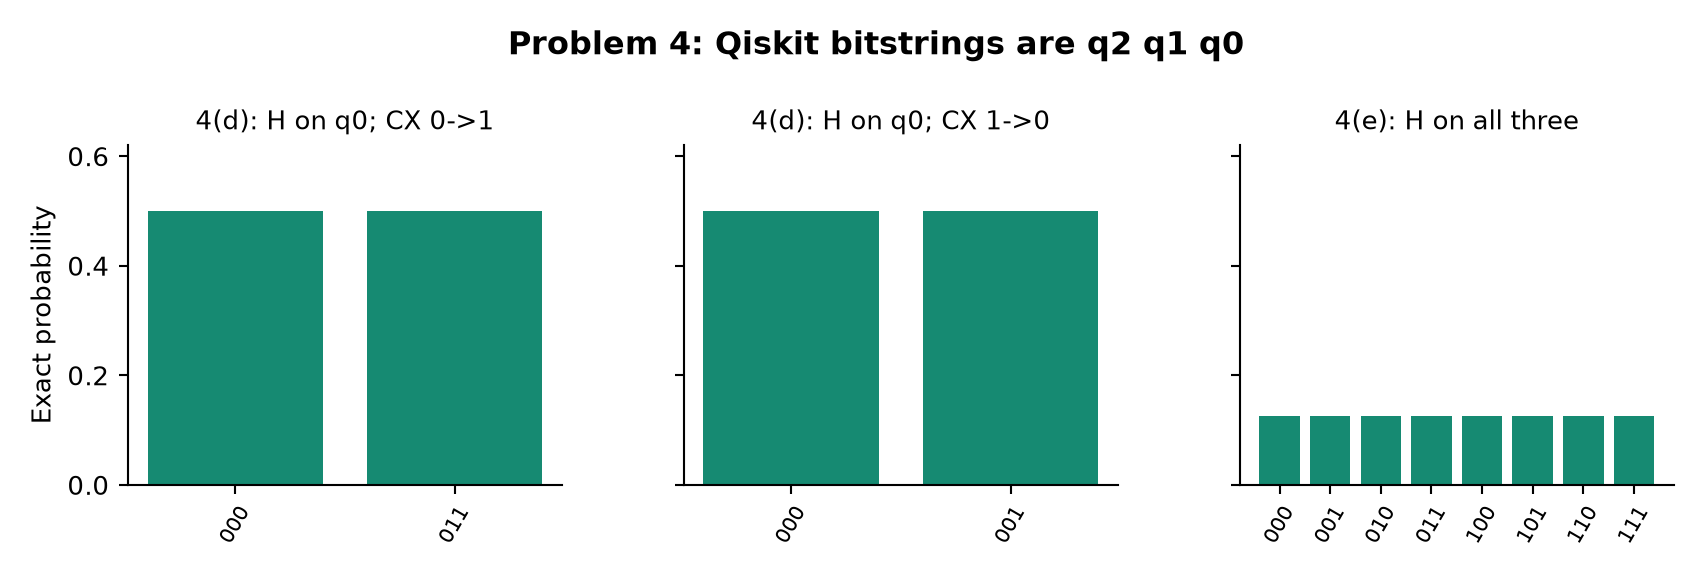
\includegraphics[width=0.92\textwidth]{./figures/problem4_circuit_outcomes.png}
\caption{Exact outcome distributions: part (d) applies H to q0 only; part (e) applies H to all three qubits.}
\end{figure}

\small
\begin{enumerate}[label=\textbf{(\alph*)},leftmargin=*,itemsep=1pt,topsep=1pt,parsep=0pt]
\item \textbf{Question.} Prove that \((H\otimes H)\ket{00}=(H\ket{0})\otimes(H\ket{0})\). Explain why this generalizes to \(n\) qubits.\\
\textbf{Answer.} Since \(H\ket{0}=(\ket{0}+\ket{1})/\sqrt2\), both sides equal \(\tfrac12(\ket{00}+\ket{01}+\ket{10}+\ket{11})\). Repeating the componentwise action proves \((\bigotimes_jU_j)(\bigotimes_j\ket{\psi_j})=\bigotimes_jU_j\ket{\psi_j}\).
\item \textbf{Question.} Explain how tensoring unitaries allows us to define operations on multi-qubit systems.\\
\textbf{Answer.} Tensor products act on the joint Hilbert space, and \((U\otimes V)^\dagger(U\otimes V)=(U^\dagger U)\otimes(V^\dagger V)=I\otimes I\). Use identity operators on wires untouched at a circuit step; a joint CNOT acts branchwise.
\item \textbf{Question.} Construct a Qiskit circuit on two qubits applying \(H\) to both, and verify it matches your result in (a).\\
\textbf{Answer.} The notebook applies H to \(q_0,q_1\) and checks the statevector \(|++\rangle\). Each computational-basis result has probability \(1/4\); the seeded 1024-shot counts were \(00:257,\ 01:255,\ 10:266,\ 11:246\).
\item \textbf{Question.} On three qubits: Case 1—apply H to \(q_0\) only, then CNOT(0\(\to\)1) (with convention being control qubit number \(\to\) target qubit number, starting qubit indexing at 0 because we count our qubits like real computer scientists). Case 2—apply H to \(q_0\) only, then CNOT(1\(\to\)0). In both cases, show mathematically (tensor product or simulation) how you can do an analogous computation to what was done in (a) for more general multi-qubit systems. Hint: if nothing is done to a qubit at a step of the quantum circuit, use the identity matrix as the quantum operation on it (the do-nothing gate). See the circuits below to get an idea of each case, following Case 1 and then Case 2; the figures show H on every qubit, but you should apply H only to \(q_0\).\\
\textbf{Answer.} Before CNOT, \((H\otimes I\otimes I)|000\rangle=(|000\rangle+|100\rangle)/\sqrt2\). Case 1 gives \((|000\rangle+|110\rangle)/\sqrt2\); Case 2 leaves \((|000\rangle+|100\rangle)/\sqrt2\) unchanged because the control \(q_1=0\). Seeded counts in Qiskit order \(q_2q_1q_0\) were Case 1: \(000:521,\ 011:503\); Case 2: \(000:521,\ 001:503\).
\item \textbf{Question.} \textit{Food for thought:} if you instead apply H to all three qubits before the CNOT (as in the figures), show that Case 1 and Case 2 produce exactly the same state. Why does the CNOT direction not matter here? (Hint: what is CNOT\(\ket{++}\)? Is \(\ket{+++}\) entangled?)\\
\textbf{Answer.} The state is the product \(|+++\rangle\). Since \(X|+\rangle=|+\rangle\), either CNOT leaves it unchanged; the two gates remain different on other inputs. The statevectors were equivalent, and both circuits produced the same seeded counts: \(000:139,\ 001:124,\ 010:127,\ 011:134,\ 100:131,\ 101:127,\ 110:124,\ 111:118\), versus exact probability \(1/8\) each.
\end{enumerate}
\normalsize
\pagereferences{(a)--(b): QML0 / Lecture 1, slides 40--43 (tensor products); (c)--(e): slides 57--61 (circuits and bit order), QML2 / Lecture 3, slides 19--20 and 24--30 (counts versus states and circuit/state reasoning).}

\newpage
\problem{Half and Full Quantum Adders}{30}\label{problem-5-half-and-full-quantum-adders}

\begin{figure}[H]
\centering
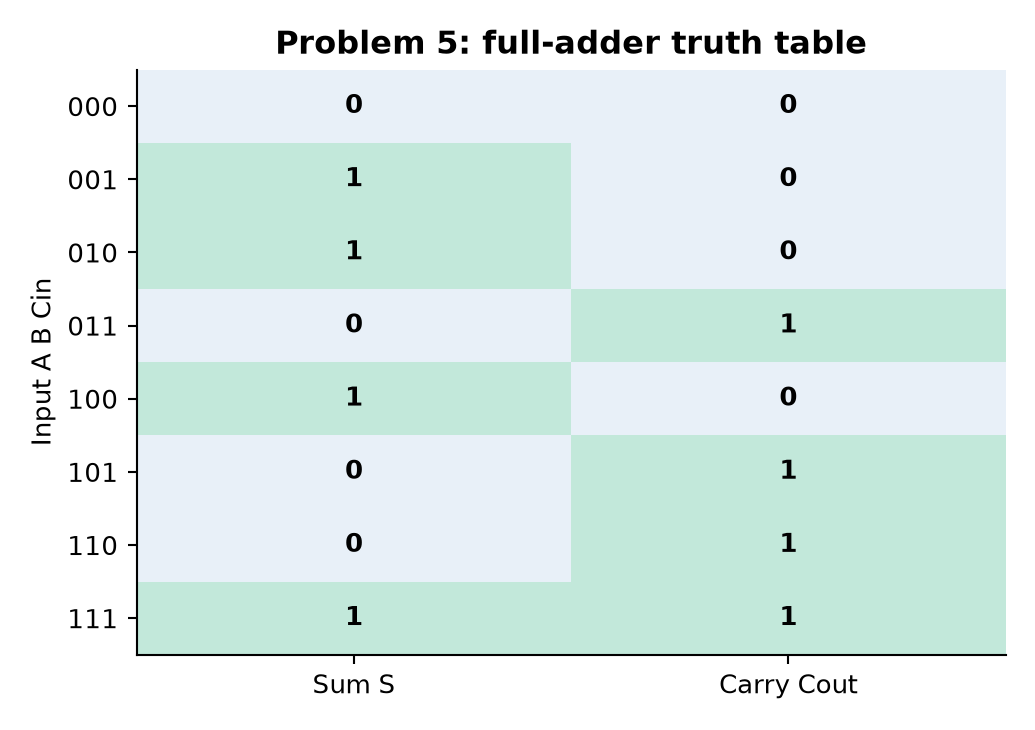
\includegraphics[width=0.64\textwidth]{./figures/problem5_full_adder_truth_table.png}
\caption{Full-adder outputs for every A, B, Cin input; the Cin=0 rows also check the half-adder outputs.}
\end{figure}

\small
\begin{enumerate}[label=\textbf{(\alph*)},leftmargin=*,itemsep=1pt,topsep=1pt,parsep=0pt]
\item \textbf{Question.} Work out by hand what happens to \(\ket{110}\) as input to the half quantum adder and \(\ket{1100}\) for the full adder. What is the final expected quantum state before measurement?\\
\textbf{Answer.} The half-adder gates CCX(0,1,2), CX(0,1) give \(\ket{110}\to\ket{111}\to\boxed{\ket{101}}\), so \(S=0,C=1\). The full-adder gates are CCX(0,1,3), CX(0,1), CCX(1,2,3), CX(1,2), CX(0,1), giving \[
\ket{1100}\to\ket{1101}\to\ket{1001}\to\ket{1001}\to\ket{1001}\to\boxed{\ket{1101}},
\] so \(S=0,C_{out}=1\). These are full register states before measurement.
\item \textbf{Question.} Implement both circuits in Qiskit, initializing carry to \(\ket{0}\) and setting inputs with \(X\) gates as needed.\\
\textbf{Answer.} The notebook follows the pinned gate order, initializes carry targets at zero, and prepares each input from \(\ket{0\cdots0}\) with conditional X gates.
\item \textbf{Question.} Run for inputs \((q_0,q_1)\in\{00,01,10,11\}\) for the half adder. Do the same with the full adder, with \(C_{in}=q_2=0\). Use conditional \(X\) gates to prepare inputs that start in the ground state on the appropriate qubit. Record outputs \((q_1,q_2)\) which represent the value of the addition and if carry is present, respectively for the half adder, and measure \((q_2,q_3)\) for the full adder, which hold \(S\) and \(C_{out}\) respectively.\\
\textbf{Answer.} Half outputs are \((S,C)=(q_1,q_2)\); full outputs are \((S,C_{out})=(q_2,q_3)\). Since \(S\to c_0\) and carry \(\to c_1\), Qiskit prints \(CS\):
\begin{center}\scriptsize
\begin{tabular}{c|c|c|c}
\textbf{Input AB} & \textbf{Expected (S,C)} & \textbf{Half counts} & \textbf{Full counts} \\
\hline
00 & (0,0) & 00:1024 & 00:1024 \\
01 & (1,0) & 01:1024 & 01:1024 \\
10 & (1,0) & 01:1024 & 01:1024 \\
11 & (0,1) & 10:1024 & 10:1024
\end{tabular}
\end{center}
\item \textbf{Question.} Compare the quantum adder results using a simulator did you find what you expected? You are in no way required to, but feel free to run this same circuit on Qiskit's real quantum computers instead of simulator - did your results change?\\
\textbf{Answer.} Ideal Aer (1024 shots, seed 739) matched all predicted outputs. With \(C_{in}=1\), inputs 001, 011, 101, 111 printed 01, 10, 10, 11, each 1024 times. No hardware run was performed; hardware is optional and may produce noisy distributions.
\end{enumerate}
\normalsize
\pagereferences{(a)--(d): QML0 / Lecture 1, slides 48, 54, and 57--62 (gate and register tracking); QML3 / Lecture 4, slide 4 (half-adder warm-up).}

\newpage
\bonus{Time-Dependent Schrödinger Dynamics and Quantum Control}{15}\label{bonus-a-time-dependent-schruxf6dinger-dynamics-and-quantum-control}

\begin{figure}[H]
\centering
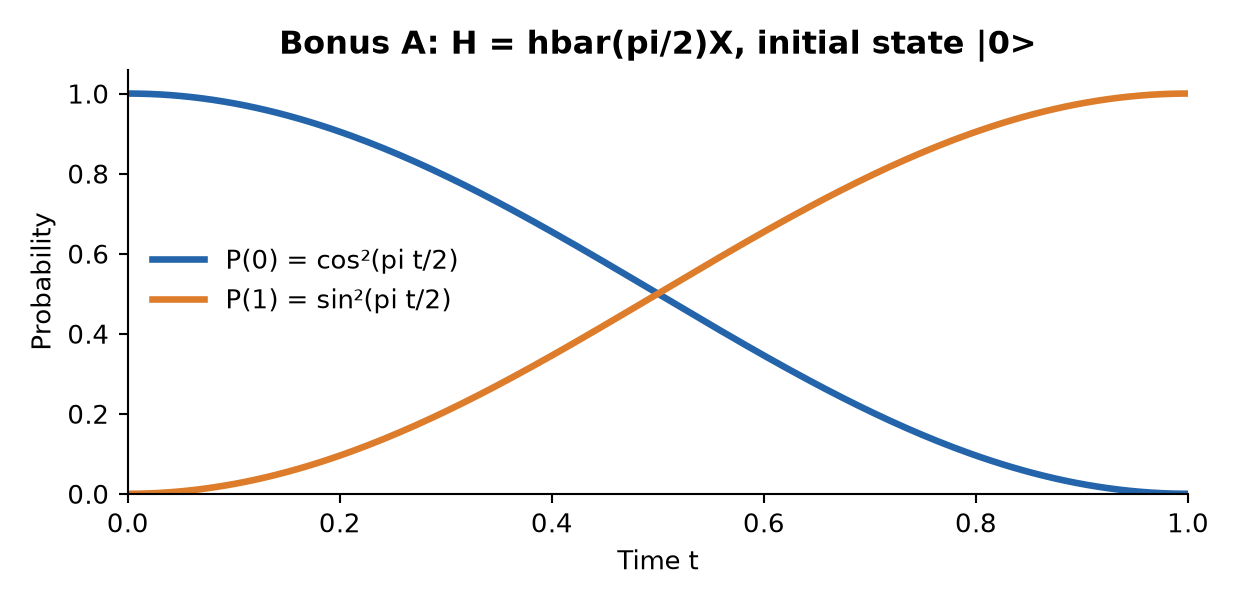
\includegraphics[width=0.70\textwidth]{./figures/bonus_a_time_evolution.png}
\caption{Example evolution from \textbar0\textgreater{} under H=\(\hbar(\pi/2)X\); the general amplitude-swap result is derived below.}
\end{figure}

\scriptsize
\textbf{Given.} The time-dependent Schrödinger equation is \(i\hbar\,d\ket{\psi(t)}/dt=H(t)\ket{\psi(t)}\), with \(\ket{\psi(0)}=\alpha\ket0+\beta\ket1\), \(\alpha,\beta\in\mathbb C\), and \(|\alpha|^2+|\beta|^2=1\). The Hamiltonian is Hermitian.
\begin{enumerate}[label=\textbf{(\alph*)},leftmargin=*,itemsep=1pt,topsep=1pt,parsep=0pt]
\item \textbf{Question.} Assume the Hamiltonian commutes with itself at different times, \([H(t),H(t')]=0\) for all \(t,t'\) (this is automatic if \(H\) is time-independent). Consider the general solution to this equation under that assumption: \(\ket{\psi(t)}=U(t)\ket{\psi(0)}\), \(U(t)=e^{-\tfrac{i}{\hbar}\int_0^tH(\tau)d\tau}\), and prove it solves the Schrödinger equation. (Without this assumption the solution is a time-ordered exponential, which is beyond the scope of this problem.)\\
\textbf{Answer.} Let \(A(t)=-(i/\hbar)\int_0^tH(\tau)d\tau\). Commutation gives \([A,A']=0\), so \(U'=A'U=-(i/\hbar)HU\). Thus \(i\hbar\,d(U\ket{\psi(0)})/dt=HU\ket{\psi(0)}\), and \(U(0)=I\) supplies the initial condition.
\item \textbf{Question.} Prove \(U(t)\) is unitary if \(H(t)\) is Hermitian. A matrix \(U(t)\) is said to be unitary if \(U^\dagger(t)U(t)=U(t)U^\dagger(t)=I\), where \(U^\dagger(t)\) denotes the conjugate transpose (Hermitian adjoint) of \(U(t)\). Unitarity guarantees that inner products and probabilities are preserved under time evolution. A matrix \(H(t)\) is said to be Hermitian if \(H^\dagger(t)=H(t)\). Hermiticity ensures that the eigenvalues of the Hamiltonian are real, so that measurable energies are real numbers.\\
\textbf{Answer.} Hermitian \(H\) makes \(A^\dagger=-A\). Therefore \(U^\dagger=e^{-A}\) and \(U^\dagger U=UU^\dagger=I\).
\item \textbf{Question.} For \(H(t)=\hbar\Omega\begin{bmatrix}0&1\\1&0\end{bmatrix}\) on \([0,1]\), compute \(U(t)\), and choose a real number \(\Omega\) so that \(U(1)\) swaps \(\alpha,\beta\) (up to a global phase). Note \(\Omega\) must be real so that \(H(t)\) stays Hermitian.\\
\textbf{Answer.} Since \(X^2=I\), \[
U(t)=e^{-i\Omega tX}=\cos(\Omega t)I-i\sin(\Omega t)X
=\begin{pmatrix}\cos\Omega t&-i\sin\Omega t\\-i\sin\Omega t&\cos\Omega t\end{pmatrix}.
\] Choose \(\Omega=\pi/2\), giving \(U(1)=-iX\) and \(\ket{\psi(1)}=-i(\beta\ket0+\alpha\ket1)\).
\item \textbf{Question.} Show \(\ket{\psi(1)}\) is normalized, e.g. the sum of the probabilities equals 1.\\
\textbf{Answer.} The probabilities are \((|\beta|^2,|\alpha|^2)\), whose sum is \(|\alpha|^2+|\beta|^2=1\).
\item \textbf{Question.} Identify the effective one-qubit gate implemented from the time evolution of the quantum system over \(t\in[0,1]\).\\
\textbf{Answer.} It is Pauli \(X\), up to the global phase \(-i\).
\end{enumerate}
\normalsize
\pagereferences{(a)--(e): QML0 / Lecture 1, slide 74 (Schr\"odinger-equation context only; the derivation is developed in the answer).}

\newpage
\bonus{Two-Bit Ripple-Carry Addition of 2 + 2}{15}\label{bonus-b-two-bit-ripple-carry-addition-of-2-2}

\begin{figure}[H]
\centering
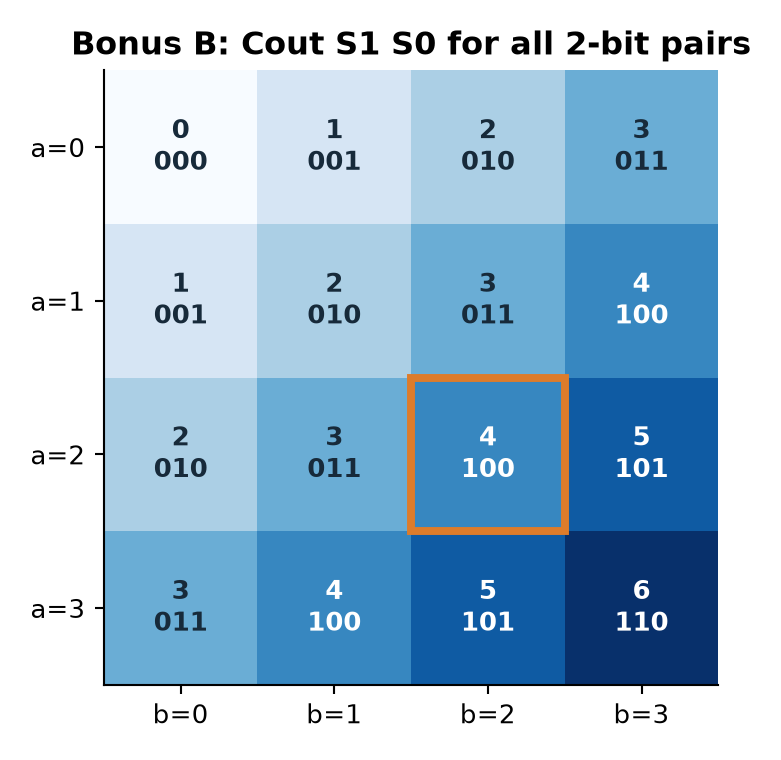
\includegraphics[width=0.58\textwidth]{./figures/bonus_b_two_bit_addition.png}
\caption{All 16 two-bit input pairs and their three-bit outputs Cout S1 S0; the orange box marks 2+2=4.}
\end{figure}

\scriptsize
\begin{enumerate}[label=\textbf{(\alph*)},leftmargin=*,itemsep=1pt,topsep=1pt,parsep=0pt]
\item \textbf{Question.} Implement a 2-bit ripple-carry adder with two 2-qubit registers \((a_1a_0,b_1b_0)\) and carry \(c\).\\
\textbf{Answer.} Map \((q_0,q_1,q_2,q_3,q_4,q_5)=(a_0,a_1,b_0,b_1,c_1,c_{out})\). The low half-adder uses CCX(0,2,4), CX(0,2); the high full adder uses CCX(1,3,5), CX(1,3), CCX(3,4,5), CX(3,4), CX(1,3). The low carry feeds the high stage.
\item \textbf{Question.} Prepare \(a=2\) and \(b=2\) in binary (\(10_2\) each), with \(c=0\).\\
\textbf{Answer.} Starting from zero, apply X to \(q_1,q_3\). In written \(q_0\cdots q_5\) order, the input is \(\ket{010100}\); both carry/work qubits start at zero.
\item \textbf{Question.} For the correct binary inputs, work through the quantum circuit (either by hand or with computer) to work out the expected result \(2+2=4=100_2\). Show how this appears as \((s_0,s_1,c_{out})\) on your qubits and as a bitstring in the Qiskit register.\\
\textbf{Answer.} The low stage gives \((s_0,c_1)=(0,0)\); the high stage gives \((s_1,c_{out})=(0,1)\). The full register trace is \(\ket{010100}\to\ket{010100}\to\ket{010101}\to\ket{010001}\to\ket{010001}\to\ket{010001}\to\ket{010101}\). Thus \((s_0,s_1,c_{out})=(0,0,1)\).
\item \textbf{Question.} Simulate and record the dominant measurement outcome.\\
\textbf{Answer.} Statevector checks match ordinary addition for all 16 two-bit input pairs. For this circuit the ideal 1024-shot Aer result (seed 739) is \texttt{100:1024}, i.e. \(100_2=4\).
\item \textbf{Question.} (Optional) Run on hardware (\(\sim 100\) shots). Compare simulator vs. noisy hardware outcomes.\\
\textbf{Answer.} No hardware run was performed; the assignment marks it optional.
\item \textbf{Question.} State clearly your measurement mapping for \((s_0,s_1,c_{out})\). Hint: follow the important point I mentioned, so you really internalize the ordering of bits in a qubit versus binary representation/register \smiley{}.\\
\textbf{Answer.} Measure \(q_2\to c_0=s_0\), \(q_4\to c_1=s_1\), and \(q_5\to c_2=c_{out}\). Qiskit prints \(c_2c_1c_0=100\), the reverse-index register string for these mapped output bits.
\end{enumerate}
\normalsize
\pagereferences{(a)--(f): QML0 / Lecture 1, slides 57--61 (circuit reading and qubit-order conventions).}

\vfill
\begin{center}
\scriptsize\textbf{AI-use statement:} AI assistance was used to review my existing written and coded work, study the course lectures and notes, map and reference relevant material for each problem and bonus, and automate preparation of this document.
\end{center}

\end{document}
